


\section{Approximations}

For some problems, it may be interesting to understand the behaviour
of these distributions for small $t$. 

\subsection{Examples}

\subsubsection{Line}
For the line \eqref{eq:line_line} we need no approximation:
\begin{equation}
  g^{\rm line}_L(t) = \frac{2}{L} - \frac{2}{L^2} t.
\end{equation}

\subsubsection{Rectangle (and square)}
For the rectangle (and square) we need only restrict our attention to
the case $t<a$ (the smaller side length), to get a simple polynomial
expression: 
\begin{eqnarray}
  g^{\rm rect}_{a,b}(t) & = & 
           \frac{4 t}{a^2 b^2}  
         \left[ \frac{ab \pi}{2} - (a+b) t + \frac{t^2}{2} \right],
          \nonumber \\
                         & = & \frac{2 \pi}{A} t 
                              - \frac{2 P}{A^2} t^2
                              + \frac{2}{A^2} t^3,
\end{eqnarray}
where $A = ab$ is the area of the rectangle, and $P = a+b$ is the perimeter.

The affect of changing the scale must be obvious, in that we know area
scales quadratically, and perimeter linearly with the size of the
region, so simple dimensional analysis suggests a form such as that
above must occur, but it is perhaps suprising that it is so clean. 

\subsubsection{Cube (and box)}
For the cube~\cite{weisstein:_cube_line_picking}, for small $t$,
\begin{eqnarray}
  g^{\rm cube}_{1}(t) & = &  -t^2 \left[ (t-8)t^2 + \pi (6 t - 4) \right], \nonumber \\
                    & = & 4 \pi t^2 - 6 \pi t^3 + 8 t^4 - t^5.
\end{eqnarray}
For the box~\cite{philip:_probab_distr_distan_between_two} with $t < a
\leq b \leq c$, we first see the distribution  of $u=t^2$ (using $g(t)
= 2 t h(t^2)$, 
\begin{eqnarray}
  h^{\rm box}_{a,b,c}(u) & = &
  \frac{1}{6 a^2 b^2 c^2} \left[
    - 6 \pi b c u + 8 b u^{3/2}
    +12 \pi a b c \sqrt u - 6 \pi a(b + c)u + 8(a + c) u^{3/2} - 3 u^2
    \right], \nonumber \\
  g^{\rm box}_{a,b,c}(t)  & = &
  \frac{t }{3 a^2 b^2 c^2} \left[
    - 6 \pi b c t^2 + 8 b t^{3}
    +12 \pi a b c t - 6 \pi a(b + c)t^2 + 8(a + c) t^{3} - 3 t^4
    \right], \nonumber \\
 & = & \frac{4 \pi}{V} t^2
       + \frac{\pi }{3 V^2} \left[ -6 b c - 6 a (b+c) \right] t^3
       + \frac{1}{3 V^2} \left[ 8 b + 8 (a+c) \right] t^4
       + \frac{1}{3 V^2} \left[ - 3 \right] t^5, \nonumber \\
 & = & \frac{4 \pi}{V} t^2
       - \frac{2 \pi }{ V^2} \left[ a b + bc + a c \right] t^3
       + \frac{8}{3 V^2} \left[ a + b + c \right] t^4
       - \frac{1}{V^2} t^5,  \nonumber \\
 & = & \frac{4 \pi}{V} t^2
       - \frac{\pi S}{ V^2} t^3
       + \frac{2 P}{3 V^2}  t^4
       - \frac{1}{V^2} t^5, 
\end{eqnarray}
for volume $V = a b c$, surface area $S = 2(a b + bc + a c)$ and edge
perimeter $P = 4(a + b + c)$>


\subsubsection{Hyperball}

For the $n$-dimensional hyperball, simple approximations are available
by use of Taylor series. Ignoring the 1D case (which is the same as
the line), we see the 2D disk
from~\cite{tu00:_circle_line,weisstein:_circle_line_picking}: 
\[
   g^{2D-{\rm ball}}_R(t) 
     =  \frac{4 t}{\pi R^2} \cos^{-1} \left( \frac{t}{2R} \right) 
               - \frac{2 t^2}{\pi R^3} \sqrt{1 - \frac{t^2}{4 R^2} }          
\]
and we use
\begin{eqnarray*}
  \cos^{-1}(x)  & = & \frac{1}{2} \pi - x - \frac{1}{6} x^{3} + \cdots \\
  \sqrt{1 - x^2} & = & 1 - \frac{x^2}{2} - \frac{x^4}{8}  + \cdots.
\end{eqnarray*}
% http://www.wolframalpha.com/input/?i=Taylor+series+of+%288%2F%28pi*R%29%29*%28x*arccos%28x%29+-+x^2*sqrt%281-x^2%29+%29
% http://www.wolframalpha.com/input/?i=Taylor+series+of+%288%2F%28pi*R%29%29*%28%28t%2F%282*R%29*arccos%28t%2F%282*R%29%29+-+%28t%2F%282*R%29%29^2*sqrt%281-%28t%2F%282*R%29%29^2%29+%29
to derive
\begin{eqnarray}
  g^{2D-{\rm ball}}_R(t) 
         & = & \frac{4 t}{\pi R^2} \cos^{-1} \left( \frac{t}{2R} \right) 
               - \frac{2 t^2}{\pi R^3} \sqrt{1 - \frac{t^2}{4 R^2} }
               \nonumber \\
         & = & \frac{4 t}{\pi R^2} \left( \frac{1}{2} \pi - \frac{t}{2R} \right)
                   -  \frac{2 t^2}{\pi R^3} + O(t^4)  \nonumber \\
         & = &  \frac{2 t}{R^2} -  \frac{4 t^2}{\pi R^3}  + O(t^4) \nonumber \\
         & = &  \frac{2 \pi}{A} t -  \frac{2 P}{A^2} t^2 + O(t^4) 
\end{eqnarray}
where once again $A=\pi R^2$ and $P = 2 \pi R$ are area and perimeter,
respectively. We note that this is very similar to the formula
obtained for the square for small $t$. The first two terms are, in
fact, identical.

For the 3D ball we already have the expression as a polynomial:
\begin{eqnarray}
  g^{3D-{\rm ball}}_R(t) 
        & = & \frac{3 t^2}{R^3} - \frac{9 t^3}{4 R^4} + \frac{3 t^5}{16 R^6}  \nonumber , \\
        & = & \frac{4 \pi}{V} t^2 - \frac{\pi S}{V^2} t^3 + \frac{3}{16 R^6} t^5,
\end{eqnarray}
where again $V=4 \pi R^3/3$ and $S = 4 \pi R^2$ are the volume and
surface area. Interestingly, these are identical to those terms for
the cube, and even the forth order term is the same if we say that the
sphere has zero edges.


%%%%%%%%%%%%%%%%%%%%%%%%%%%%%%%%%%%%%%%%%%%%%%%%%%%%%%%%%%%%%%%%%%5


The more general expression for the $n$-D ball can be derived by
noting that for a $n$-dimensional ball of radius $R$,
\begin{equation}
 g^{nD-{\rm ball}}_R(t) = n \frac{t^{n-1}}{R^n} I_x\left( 
  \frac{1}{2} (n+1), \frac{1}{2}
                      \right),
\end{equation}
rememeber $x = 1 - t^2/4R^2$, $a=(n+1)/2$, and $b=1/2$, and from
\cite[26.5.4]{Abramowitz_and_Stegun}
\begin{eqnarray}
  \label{eq:Ix}
  I_x(a,b) 
 & = & 1 - I_{1-x}(b,a)
                    \nonumber \\
 & = & 1 - \frac{(1-x)^b x^a}{b B(b,a)}  \left\{ 
               1 +
               \sum_{i=0}^{\infty} \frac{B(b+1,i+1)}{B(a+b,i+1)} (1-x)^{i+1}
           \right\} 
               \nonumber \\
 & = & 1 - \frac{2 (t/2R) (1 - t^2/4R^2)^a}{B(b,a)}  \left\{ 
               1 +
               \sum_{i=0}^{\infty} \frac{B(b+1,i+1)}{B(a+b,i+1)} (t/2R)^{2(i+1)}
           \right\} 
               \nonumber \\
 & \simeq & 1 - \frac{t/R}{B(b,a)} 
               + \frac{a t^3/4R^3 }{B(b,a)} 
               - \frac{2 (t/2R)}{B(b,a)} \frac{B(b+1,1)}{B(a+b,1)} (t/2R)^{2}
               \nonumber \\
 & \simeq & 1 - \frac{t/R}{B(1/2,(n+1)/2)} 
               + \frac{1}{4 B(1/2,(n+1)/2)} 
                   \left[ \frac{n+1}{2}
                          -\frac{B(3/2,1)}{B(n/2+1,1)} \right] (t/R)^{3}.
\end{eqnarray}
The Gamma function satisfies\cite[6.1.12]{Abramowitz_and_Stegun}
\begin{eqnarray}
  \label{eq:gamma}
  \Gamma(1/2) & = & \pi^{1/2}, \\
  \Gamma(3/2) & = & \frac{1}{2} \pi^{1/2}, \\
  \Gamma(k+1) & = & k!, \\
  \Gamma(k+1/2) & = & \frac{(2k)! \pi^{1/2}}{2^{2k} k!},
\end{eqnarray}
% last one comes from Wiki, but could be derived simply from A&S
so we can derive
\begin{eqnarray}
  \label{eq:beta_specified_vals}
  B(1/2,(n+1)/2) & = & \frac{\Gamma(1/2) \Gamma((n+1)/2)}{\Gamma(n/2 + 1)} \nonumber \\
  & = & \left\{ \begin{array}{ll}
      \displaystyle \frac{\pi^{1/2} \Gamma(k)}{\Gamma(k+1/2)} & n \mbox{ odd, i.e., } n=2k-1,\\
      \displaystyle \frac{\pi^{1/2} \Gamma(k+ 1/2)}{\Gamma(k + 1)} & n \mbox{ even, i.e., } n=2k.\\
    \end{array} \right. \nonumber \\
  & = & \left\{ \begin{array}{ll}
      \displaystyle \frac{\pi^{1/2} 2^{2k} k! (k-1)!}{(2k)! \pi^{1/2}} & n \mbox{ odd, i.e., } n=2k-1,\\
      \displaystyle \frac{\pi^{1/2} (2k)! \pi^{1/2}}{2^{2k} k! k!} & n \mbox{ even, i.e., } n=2k.\\
    \end{array} \right. \nonumber \\
  & = & \left\{ \begin{array}{ll}
      \displaystyle \frac{2^{2k} k! (k-1)!}{(2k)! } & n \mbox{ odd, i.e., } n=2k-1,\\
      \displaystyle \frac{\pi (2k)!}{2^{2k} k! k!} & n \mbox{ even, i.e., } n=2k.\\
    \end{array} \right.
\end{eqnarray}
Thus the asymptotic form of these distributions for $t
\rightarrow 0$, i.e., 
\begin{equation}
  \label{eq:asympt_line_picking}
  g^{nD-{\rm ball}}_R(t) = n \frac{t^{n-1}}{R^n} + 
    n \frac{t^{n}}{R^{n+1}} 
   \left\{ \begin{array}{ll}
      \displaystyle 
           \frac{(2k)! }{2^{2k} k! (k-1)!} & \mbox{ for } n=2k-1,\\
      \displaystyle 
           \frac{2^{2k} k! k!}{\pi (2k)!} & \mbox{ for } n=2k.\\
    \end{array} \right\}
 +  O(t^{n+1}).
\end{equation}
For example: when $n=1,2,3$ and $4$:
\begin{eqnarray}
  \label{eq:ex_g(t)}
g^{1D-{\rm ball}}_R(t)
 & \simeq &                        
  n \frac{t^{n-1}}{R^n} - 
    n \frac{t^{n}}{R^{n+1}} 
   \left\{  \frac{(2k)! }{2^{2k} k! (k-1)!}  \right\},
                 \;\;\; \mbox{ where $n$ is odd, and } k=1,  \nonumber \\
 & \simeq &                          % (k=1, n odd)
  \frac{1}{R} - 
    \frac{1}{2} \frac{t}{R^{2}}. 
                 \\
g^{2D-{\rm ball}}_R(t)
 & \simeq &                          % (k=1, n even)
  n \frac{t^{n-1}}{R^n} - 
    n \frac{t^{n}}{R^{n+1}} 
   \left\{ \frac{2^{2k} k! k!}{\pi (2k)!}  \right\},
                 \;\;\; \mbox{ where $n$ is even, and } k=1,  \nonumber \\
 & \simeq &                          % (k=1, n even)
  2 \frac{t^{1}}{R^2} - 
    \frac{4}{\pi} \frac{t^{2}}{R^{3}} .
                  \\
g^{3D-{\rm ball}}_R(t)
 & \simeq &                          % (k=2, n odd)
  n \frac{t^{n-1}}{R^n} - 
    n \frac{t^{n}}{R^{n+1}} 
   \left\{ \frac{(2k)! }{2^{2k} k! (k-1)!}  \right\},
                 \;\;\; \mbox{ where $n$ is odd, and } k=2,  \nonumber \\
 & \simeq &                          % (k=2, n odd)
  \frac{3 t^{2}}{R^3} - 
     \frac{9}{4} \frac{t^{3}}{R^{4}} .
   \\ 
g^{4D-{\rm ball}}_R(t)
 & \simeq &                          % (k=2, n even)
  n \frac{t^{n-1}}{R^n} -  
    n \frac{t^{n}}{R^{n+1}} 
   \left\{ \frac{2^{2k} k! k!}{\pi (2k)!} \right\},
                 \;\;\; \mbox{ where $n$ is even, and } k=2, \nonumber \\
 & \simeq &                          % (k=2, n even)
  \frac{4 t^{3}}{R^4} -  
    \frac{2^5}{3\pi} \frac{t^{4}}{R^{5}} .
\end{eqnarray}
which obviously agree with the previous formula. We can also calculate
the third term in the expansion, which in the case of the 3D ball
(where the density is completely given by three terms) gives the
previous formula.


The generalized volume and surface are of the $n$-D hyperball are
\begin{eqnarray}
 V_n(R) & = & C_n R^n,
  \label{eq:gen_vol} \\
 S_{n}(R) & = & \frac{dV_n}{dR} = n C_n R^{n-1}.
  \label{eq:gen_surf}
\end{eqnarray}
where
\begin{equation}
  \label{eq:cn}
   C_n = \frac{ \pi^{n/2} }{\Gamma(n/2 + 1)},
\end{equation}


%%%%%%%%%%%%%%%%%%%%%%%%%%%%%%%%%%%%%%%%%%%%%%%%%%%%%%%%%%%%%%%%%%5

\subsection{General pattern}

It seems as if there is a general pattern here.  That makes a good
deal of sense because for small $t$, the boundaries have little
affect. Hence, we would expect the shape of the region to only affect
the (small) line lengths through macro-properties such as the area and
perimeter.

\subsubsection{2D case}

Formally, consider a convex region in 2D, for $t$ small, we might
first assume that a random point is unlikely to be within distance $t$
of the boundary of the region, and so the probability density
function, to first order, is simply the probability that the second
point lies on the circle around this of radius $t$.
\begin{equation}
  g(t) \sim \frac{2 \pi}{A} t, 
\end{equation}

We can obtain a more accurate approximation by again assuming $t$ is
small, so that we can approximate the boundary by a straight line. In
this case, imagine the initial point was chosen (at random) to lie
with distance $t/2$ of the boundary. We can see that we over-estimate
the possible second points that lie at distance $t$. We can correct by
subtracting the number of such points that would actuall lie outside
the region.

Formally, in 2D, consider the first point lies at distance $\ell<t$
from the boundary, then there will be an arc of the circle of radius
$t$ that lies outside the circle (see
Figure~\ref{fig:perimeter}). Then the length of the arc in question
will be
\begin{equation}
  \label{eq:arc_len}
  s = 2 \theta = 2 \cos^{-1} (\ell / t).
\end{equation}
We then have to integrate over the possible distances $\ell$, i.e., 
\begin{eqnarray}
  \label{eq:correction_2nd_order}
   h(t) & = & \int_0^t 2 \cos^{-1} (\ell / t)  \, d\ell \nonumber \\
        & = &  - 2 t \int_{\pi/2}^0 \theta  \sin \theta \, d\theta  \nonumber \\
        & = &  2 t \int^{\pi/2}_0 \theta  \sin \theta \, d\theta  \nonumber \\
        & = &  2 t \left\{ \left[ -\theta  \cos \theta \right]^{\pi/2}_0 + 
                      \int^{\pi/2}_0  \cos \theta \, d\theta
                   \right\}  \nonumber \\
        & = &  2 t \left[ \sin \theta \right]^{\pi/2}_0  \nonumber \\
        & = &  2 t,
\end{eqnarray}
using the substitution $\theta = \cos^{-1} (\ell / t)$, or $\ell = t
\cos(\theta)$, so that $d \ell = - t \sin \theta$, and we integate by
parts. This must be multiplied by the probability that the first point
lies in the boundary region --- the area of the boundary divided by the
total boundary, i.e., $t P/A$, and divided by $A$ again to get the
probability that the second point would lie on the arc, if there were
no boundary, so the corrected form of $g(t)$ in 2D is
\begin{equation}
  g(t) \sim  \frac{2 \pi}{A} t - \frac{2 P}{A} t^2,
\end{equation}
which again matches the results for the rectangle and disk.

\begin{figure}[tbp]
  \begin{center}
    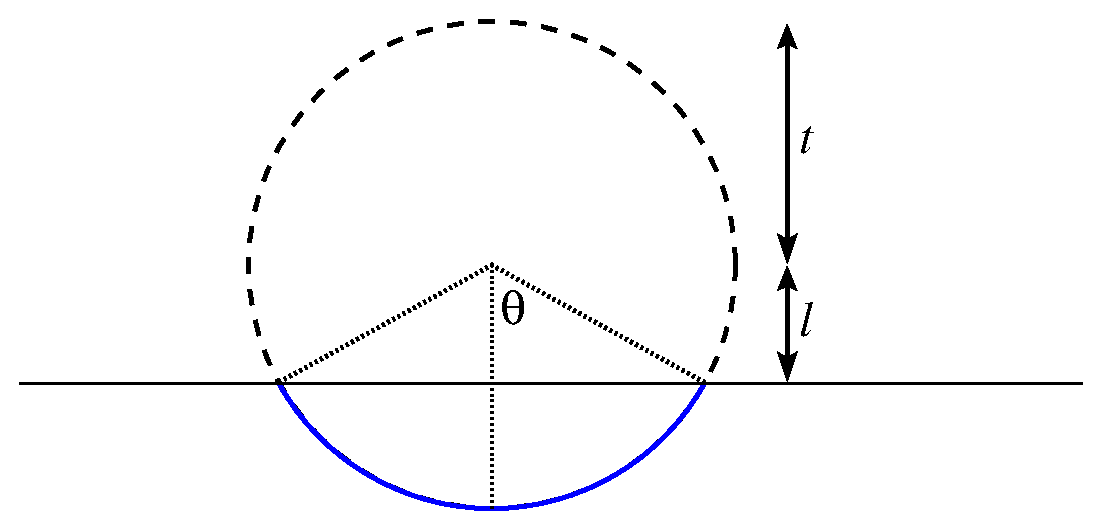
\includegraphics[width=0.33\columnwidth]{Figs/perimeter.eps}
    \caption{.}
    \label{fig:perimeter}
  \end{center} 
\vspace{-4mm}
\end{figure}

The next order correction would then build in the fact that the border
is not straight, e.g., in the case of a disk it is round, and in the
case of the square it has corners. However, as this term is very
dependent on shape and not general characteristics we won't calculate
it here.




\subsubsection{3D case}

Likewise for a region of 3D Euclidean space, we look at the
probability that the point lies on the surface of a sphere of radius
$t$, i.e.,
\begin{equation}
  g(t) \sim \frac{4 \pi}{V} t^2, 
\end{equation}
We can naturally generalize to $n$-D Euclidean spaces, by noting that
the generalized surface are of the $n$-D hyperball is
\begin{equation}
  \label{eq:surface_hyperball}
  S_{n} = \frac{dV_n}{dR} = n C_n R^{n-1}.
\end{equation}
where $V_n$ is its volume, and $C_n$ is defined in \eqref{eqn:cn}, so
the first order term of any expansion (for small $t$) of the density
function will take the form
\begin{equation}
  g(t) \sim \frac{n C_n}{V} t^{n-1}, 
\end{equation}
where $V$ is the $n$-D volume of the region of interest.

However, calculating the integral for the next term (correcting for
the perimeter would be tiresome, and in any case will be derived below.

\subsubsection{Higher dimensions}

We can go through exactly the same process in higher dimensions, to
obtain the same types of approximations, but computing the integrals
is somewhat redundant as we can see the correct forms of
approximatiosn directly from the hyperball distribution. Intuitively,
in high dimensions, the points are spread ``more thinly'' in the sense
that their density on $n$-dimensional volumes will be lower, and
hence, the distances between points will be larger. In particular the
chance of very short lines decreases, and we see this in the fact that
the first non-zero term in the Taylor series above has order $n-1$ for
the $n$-dimensional problem.

By the previous argument, we know that the result for the ball should
extend to arbitrary shapes, where $S_n$ is the general form of the
surface area, and $V_n$ the arbitrary form for the volume, so we could
for instance estimate the formula for small $t$ for a 4-rectangle with
sizes $a,b,c$ and $d$ as
\begin{eqnarray}
  g^{4D-{\rm rectangle}}_{a,b,c,d}(t)
 & \simeq  & 
      \frac{n C_n}{V_n} t^{n-1}
    -  \frac{ \pi^{(n-1)/2} }{\Gamma((n+1)/2)}
        \frac{S_n}{ V_n^2} t^{n} \nonumber \\
 & \simeq  & 
      \frac{2 \pi^{2}}{ a b c d} t^{3}
      -  \frac{8 \pi(abc + a b d + a c d + b c d)}{ 3 (a b c d)^2} t^{4}.
\end{eqnarray}



%%%%%%%%%%%%%%%%%%%%%%%%%%%%%%%%%%%%%%%%%%%%%%%%%%%%%%%%%%%%%%%%%%5

\subsection{Non-Euclidean Problems}

We can extend some of this insight into other problems, for instance,
the {\em circle line picking} problem, where pairs of points are
chosen on a circle, but the lines cross the circle. Here, the
probability distribution for line length (with a unit circle) is
\cite{weisstein:_circle_line_picking}
% http://mathworld.wolfram.com/CircleLinePicking.html
\begin{equation}
  \label{eq:circle_line_picking}
  g(t) = \frac{1}{\pi} \left(    
           1 - \frac{t^2}{4}
               \right)^{-1/2} 
       \simeq \frac{1}{\pi} \left( 1 - \frac{t^2}{4} + \cdots \right) 
\end{equation}
which is correct using the form above with $n=1$, i.e.,
\begin{equation}
  g(t) \simeq \frac{1 C_1}{2 \pi} t^0 =  \frac{1}{\pi}
\end{equation}
because $C_1=2$ and the circle, effectively has no edges.

For the {\em sphere line
  picking}~\cite{weisstein:_sphere_line_picking}, the distribution
takes the form
\begin{equation}
  g(t) \simeq \frac{1}{2} t.
\end{equation}
which works for $n=2$ and zero perimeter on the edges:
\begin{equation}
  g(t) \simeq \frac{2 \pi}{A} t = \frac{2 \pi}{4 \pi} t = \frac{1}{2} t.
\end{equation}


